\clearpage
\section[Comment explorer les données de SimFeodal ?]{Comment explorer les données de SimFeodal ?%
\sectionmark{Explorer les sorties}}\label{sec:explorer-sorties-simfeodal}

	Pour évaluer, de manière approfondie, une expérience d'un modèle tel que SimFeodal, il est nécessaire de passer en revue de nombreux indicateurs de sortie de simulation.
	Cette évaluation ne vise pas à produire une \og note\fg{} unique et synthétique, mais plutôt à tester la capacité de l'expérimentation à reproduire les dynamiques que le modèle chercher à reproduire.
	Il ne s'agit donc pas, à proprement parler, d'une évaluation du modèle, au sens quantitatif où on pourrait l'entendre, mais plutôt d'une exploration de son comportement en fonction des mécanismes et valeurs de paramètres choisis, aboutissant donc sur un jugement qualitatif sur la validité du modèle.
	Pour mener cette exploration, il convient d'utiliser des outils adaptés, c'est-à-dire de disposer de solutions techniques permettant le calcul et l'affichage des indicateurs à partir des données produites par le modèle.
	
	Dans le travail mené autour de SimFeodal, plusieurs solutions ont été utilisées au cours des différentes étapes de construction du modèle.
	La restitution purement chronologique de ces solutions ne revêt pas d'intérêt propre, mais les contraintes accumulées au cours de la construction du modèle ainsi que les choix devant permettre de les dépasser nous paraissent très largement génériques et généralisables.
	
	La succession de choix d'outils d'explorations se justifie par les verrous dans l'exploration que chacun a permis de débloquer.
	Cela dresse par là-même un portrait des solutions méthodologiques d'exploration de données de simulations dont on peut faire usage selon les contraintes générales des modèles.

	\subsection{Observation en direct vs a posteriori}\label{subsec:observation-a-posteriori}

	Classiquement, le premier réflexe d'un modélisateur, du moins pour les modèles à base d'agents, est de définir des sorties graphiques pour accompagner son modèle.
	Les différentes plate-formes de modélisation agent mettent d'ailleurs régulièrement en avant les possibilités de représentations qu'offrent leurs environnements (\hl{ref blogs Gama, NetLogo 3D, GeoMASON, Repast}).
	Visualiser le déroulement d'un modèle \og en direct\fg{} (\og \textit{online}\fg{} dans \cite{grignard_agent-based_2017}), c'est-à-dire au sein de la plate-forme de simulation et au cours l'exécution du modèle, offre ainsi de nombreux avantages : évaluation visuelle du niveau de ségrégation (et de son évolution) dans une implémentation du modèle de Schelling ; visualisation de cohérence du déplacement des nuées d'oiseaux dans un modèle de type \og Flocks\fg{} \autocite{reynolds_flocks_1987} ; ou encore suivi d'un indicateur dans le temps -- la quantité de ressources collectées -- dans un modèle de type \og Sugarscape\fg{} \autocite{epstein_growing_1996}.

	Dans l'exploration de SimFeodal, la création en direct de quelques graphiques correspondant à des indicateurs étudiés permet d'assurer un rôle de pré-filtrage au lancement des simulations et réplications associées : 
	après une modification du code-source du modèle, et avant de lancer de nombreuses simulations, on exécute quelques simulations \og manuellement\fg{}, en s'assurant, en direct, que les indicateurs affichés ne présentent pas de caractères aberrants.
	Cela permet de vérifier, avant de lancer des calculs plus intensifs, que le déroulement de la simulation semble cohérent, c'est-à-dire, le plusn souvent pour des modifications mineurs du modèle,  qu'un \textit{bug} n'a pas été introduit involontairement.
	
	Le recours à ce type de visualisation en direct des simulations ne peut toutefois être généralisé, c'est-à-dire sorti de son rôle de pré-filtre, en raison de deux principales contraintes.

	La première contrainte, déjà évoquée plus haut, est que le modèle SimFeodal est fortement stochastique.
	Dès lors, la visualisation des indicateurs d'une simulation particulière nn'est pas suffisante pour estimer le comportement du modèle.
	En conséquence, les indicateurs choisis pour l'évaluation de SimFeodal prennent presque tous en compte la variabilité des résultats induite par l'exécution de réplications.
	Certains environnements techniques (\hl{ref à multi-simulation dans Gama}) permettent toutefois de mener concomitamment plusieurs réplications d'un même modèle et de visualiser directement pendant l'exécution les résultats agrégés des réplications.
	La première contrainte, liée à l'importante étude des réplications du modèle, peut donc être dépassée en adaptant l'implémentation du modèle pour faire usage de ces capacités de multi-simulation.

	La seconde contrainte est cruciale dans le cas de SimFeodal et invalide l'usage des méthodes de visualisation en direct.
	On l'a vu, l'exploration des sorties de simulation du modèle repose sur la consultation systématique de plusieurs indicateurs, dont le nombre peut se révéler important pour une analyse approfondie.
	
	Tout d'abord, il est concrètement difficile de représenter tous ces indicateurs au sein de l'interface graphique d'une plate-forme de simulation agent, comme on peut le remarquer, par exemple en \cref{fig:simfeodal_gui_indicateurs} : l'espace occupé par les quelques indicateurs temporels et numériques affichés est déjà important et rend l'interface d'ensemble complexe.
	De plus, et c'est sans doute le verrou majeur, la temporalité de l'exécution d'une simulation -- ou même des réplications nécessaires -- est bien plus courte que celle requise pour la compréhension des résultats produits.
	Une simulation requiert ainsi au maximum quelques minutes, et pour pouvoir examiner tous les indicateurs pendant cette durée, il serait nécessaire de mettre la simulation en pause régulièrement, presque à chaque pas de temps, pour disposer d'un temps suffisant à l'observation des indicateurs (organisés en onglets dans l'interface visible dans la \cref{fig:simfeodal_gui_indicateurs}).
	Les indicateurs de sortie de simulation demandent en effet un examen approfondi pour être en mesure de juger de leur adéquation aux attentes thématiques.
	
	Cette contrainte est renforcée par la pratique d'évaluation que chaque chercheur mobilisera.
	Le plus souvent, parce que l'évaluation n'est pas une étape unique et finie, il est utile de pouvoir revenir sur les résultats à différents moments.
	Cela est par exemple nécessaire quand il s'agit de comparer de nouveaux résultats produits à ceux générés par des expérimentations antérieures.
	On ne peut alors se contenter d'évaluations en direct, même en y consacrant un temps important, simplement parce que par nature, ces évaluations seront à reproduire en plusieurs occasions, et qu'il ne serait alors pas rationnel de relancer, à chaque fois, de nouvelles simulations correspondant à des configurations de paramètres et de mécanismes déjà éprouvées.
	
	Un dernier élément accroît encore la difficulté à se baser sur une évaluation en direct : en plus du chercheur, amené à revenir de multiples fois sur les résultats d'une expérience, un modèle co-construit, qui plus est en situation d'interdisciplinarité, peut être évalué par plusieurs chercheurs différents, chacun amenant un point de vue propre.
	Sauf à faire preuve d'une discipline exacerbée, par exemple en réalisant l'ensemble du travail d'évaluation uniquement en séances de travail simultanées et collectives, l'évaluation par plusieurs personne demande que chacun puisse mener ces analyses selon ses propres temporalités et itérations.
	En choisissant de baser l'évaluation d'un modèle uniquement sur une analyse en direct, il faudrait alors que chaque chercheur, à chaque fois qu'il souhaite évaluer une même expérience, ré-exécute le modèle de nombreuses fois.
	Cela serait naturellement possible, mais constituerait clairement un gâchis certain de ressources.
	
	L'évaluation de SimFeodal ne peut donc que difficilement être réalisé en direct, qui plus est quand elle demande de faire appel, dans un cadre de co-construction, à plusieurs points de vue hétérogènes.
	Les modalités mêmes de l'exploration des sorties d'un modèle à évaluation visuelle requièrent donc que les indicateurs soient visibles et explorables à des temporalités différentes, par des chercheurs différents, depuis des lieux divers.
	
	Il est donc indispensable que les indicateurs soient enregistrés et consultables simplement à tout moment, ce qui élimine de fait la visualisation des indicateurs en direct pendant l'exécution des simulations comme unique méthode d'exploration du comportement de SimFeodal.
	
	
	\begin{figure}[H]
		\captionsetup{width=\linewidth}
		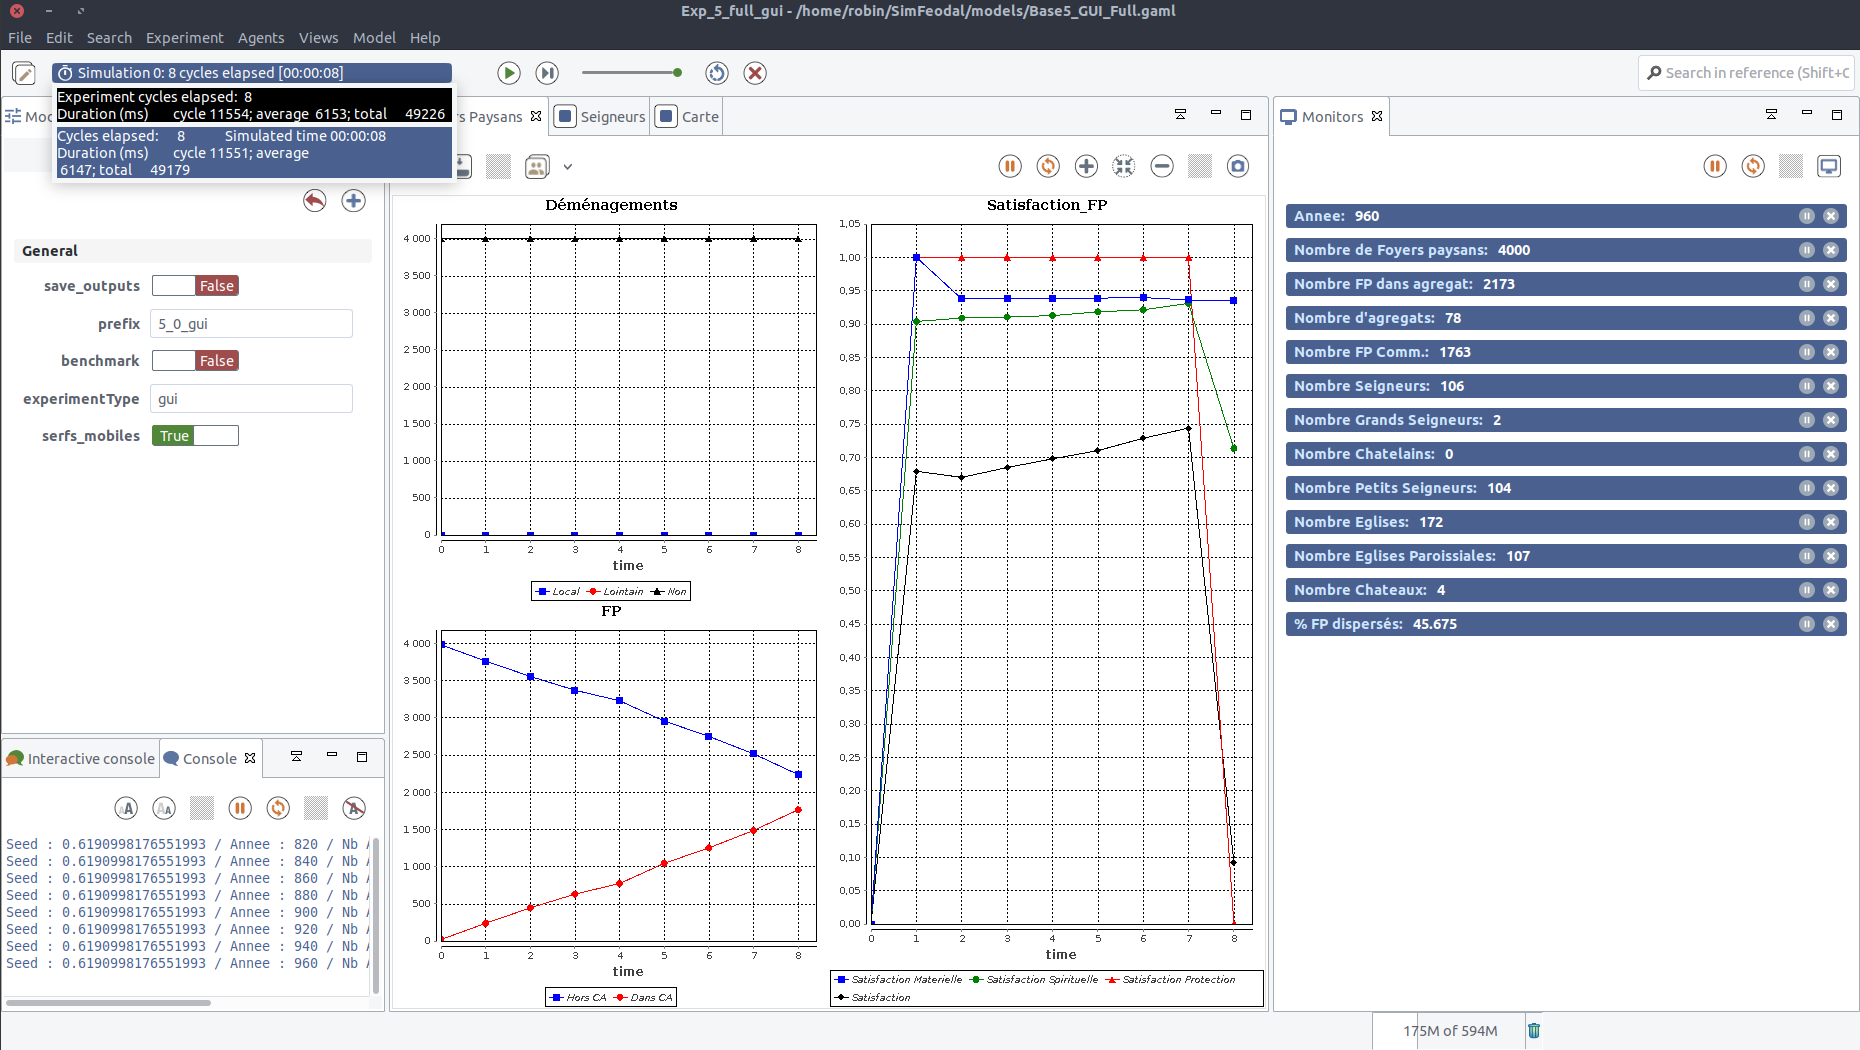
\includegraphics[width=\linewidth]{img/SimFeodal_GUI_FP.png}
		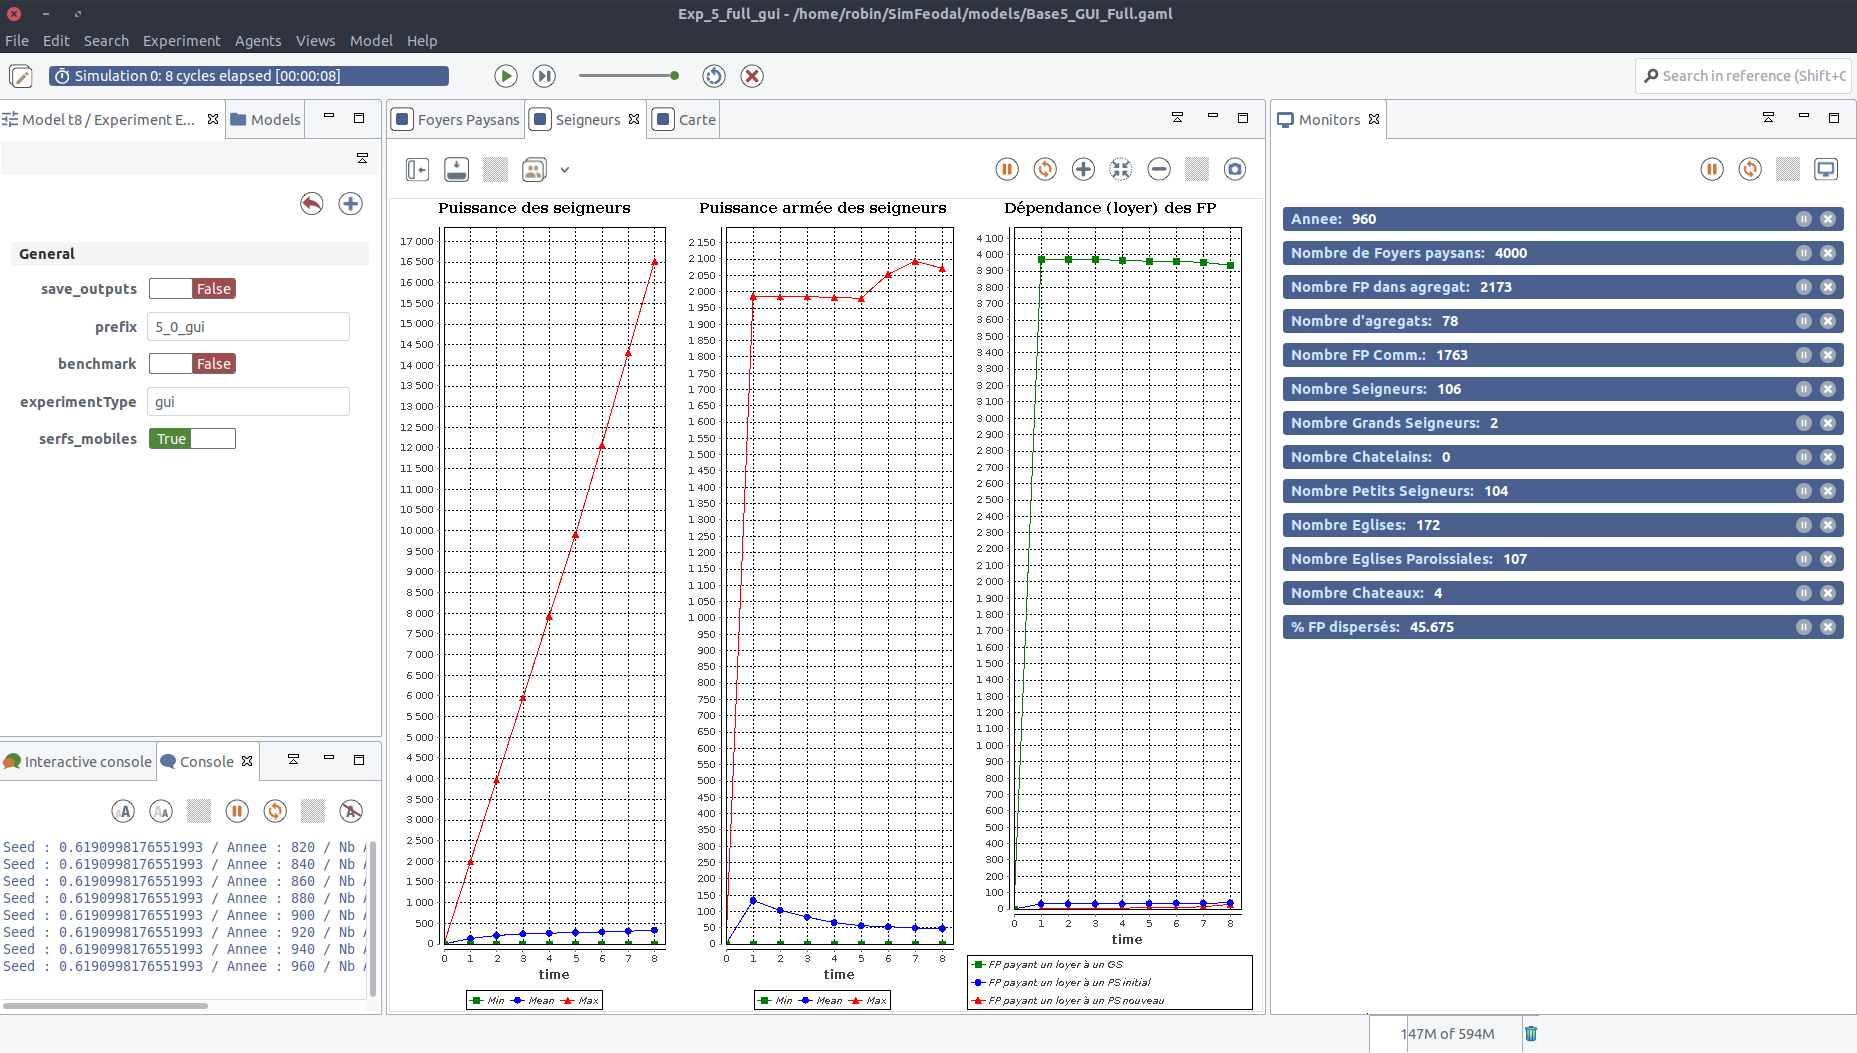
\includegraphics[width=\linewidth]{img/SimFeodal_GUI_seigneurs.png}
		\caption{Visualisations intégrées à l'interface graphique de SimFeodal : indicateurs liés aux foyers paysans et aux seigneurs.}
		\label{fig:simfeodal_gui_indicateurs}
	\end{figure}
	
	La visualisation en direct n'est donc pas mobilisable en tant que méthode d'évaluation principale, mais elle peut tout de même, comme dans un usage très classique, être utilisée comme un outil de validation interne pour tester chaque modification dans les valeurs de paramètres, remplissant alors le rôle de \og préfiltre\fg{} décrit auparavant.
	Visualiser une seule simulation, avant d'en exécuter les réplications nécessaires, permet ainsi déjà de vérifier que les modifications apportées dans les valeurs de paramètre ou dans les mécanismes n'ont pas entraîné l'apparition de \textit{bugs} ou d'incohérences immédiatement visibles.

	Nous avons donc choisi de doter SimFeodal d'une interface graphique, très sommaire, mais permettant des allers-retours rapides entre l'implémentation et l'exécution.
	Cette interface n'affiche qu'un nombre réduit d'indicateurs (\autoref{fig:simfeodal_gui_indicateurs}), ainsi qu'une représentation cartographique (\autoref{fig:simfeodal_gui_carte}) utile à une analyse rapide du comportement d'ensemble du modèle.

\begin{figure}[H]
	\captionsetup{width=\linewidth}
	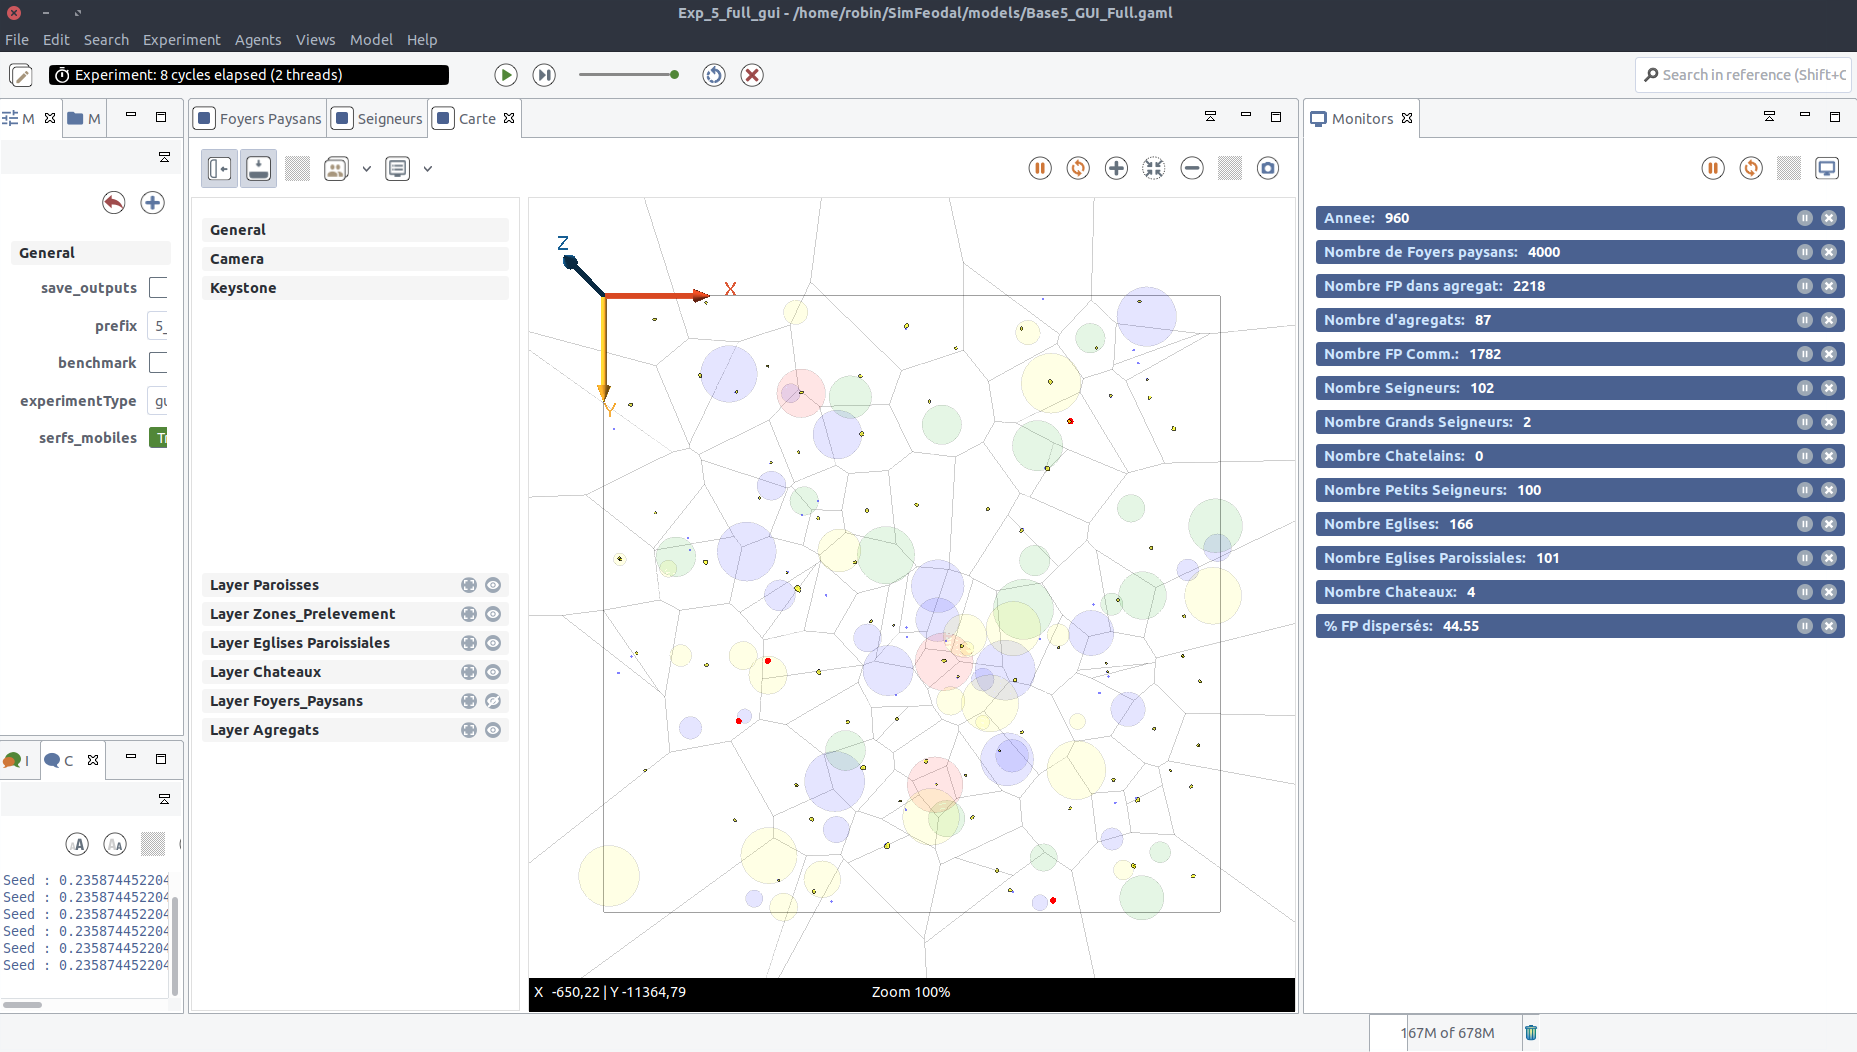
\includegraphics[width=\linewidth]{img/SimFeodal_GUI_carte.png}
	\caption{Visualisations intégrées à l'interface graphique de SimFeodal : cartographie synthétique de l'espace modélisé.}
	\label{fig:simfeodal_gui_carte}
\end{figure}

	Ces représentations, on l'a expliqué, ne suffisent pas à évaluer SimFeodal, et ne remplissent en aucun cas ce rôle : elles complètent la démarche d'évaluation du modèle par l'ajout d'une étape de contrôle préalable -- un pré-filtrage -- au lancement d'expériences. L'ajout de cette étape vient donc renforcer l'outillage d'évaluation de SimFeodal.

	\subsection{Générer les indicateurs}

	Si la production des indicateurs doit donc nécessairement être réalisée en aval de l'exécution des simulations (\og \textit{offline}\fg{} dans \cite{grignard_agent-based_2017}), il faut pour cela disposer d'outils adaptés au traitement des données produites, c'est-à-dire répondant aux contraintes identifiées auparavant (\autoref{subsec:donnees-indicateurs}).
	La contrainte principale est d'être en mesure de gérer la masse de données produites.
	On l'a vu, cela élimine d'office les outils de type tableurs, ou encore les outils de manipulation graphique de données les plus courants.
	Pour les raisons évoquées dans le chapitre 1 (\hl{Positionnement : pourquoi utiliser des outils libres ?}), seules les solutions techniques libres étaient envisageables.

	Certains outils graphiques, basés sur des logiciels libres en arrière-plan (PSPP, R Commander, Orange), sont extrêmement aisés à prendre en main et auraient pu constituer un bon choix.
	Pourtant, avec une trentaine d'indicateurs à produire pour chaque expérience, donc de manière régulière, nous avons préféré nous tourner vers des outils plus orientés vers une interface en ligne de commande (\textit{Command Line Interface}, abrégés \textit{CLI}).

	L'utilisation de CLI a plusieurs intérêts gravitant autour de la reproductibilité des traitements.
	En premier lieu, ils permettent une adaptation aisée et rapide aux différents jeux de données.
	Ainsi, partant du principe que les données générées par les réplications et expérimentations sont de même structures, il suffit généralement de modifier le chemin d'entrée des fichiers résultants pour reproduire à l'identique une analyse sur un nouveau jeu de données.

	De manière plus technique et interne à la génération des indicateurs, on peut remarquer que les différents indicateurs de sortie de simulation choisis présentent souvent des caractéristiques communes, aussi bien dans le traitement nécessaire que dans les formats (graphiques) produits.

	Par exemple, la grande majorité des indicateurs reposent sur une première agrégation des données par réplication et pas de temps simulé, puis par une seconde agrégation montrant la variabilité des situations générées, au niveau de l'expérimentation\footnote{
	On peut considérer ces agrégations comme une succession d'opération imbriquées : pour montrer l'évolution d'un indicateur tel que le taux de foyers paysans dispersés au cours du temps simulé, il faut (1) calculer le ratio entre nombre de foyers paysans dispersés et nombre total de foyers paysans, (2) pour chacun des pas de temps simulé, (3) pour chaque simulation, (4) pour l'ensemble des réplications d'une expérience, (5) éventuellement pour chacune des expériences d'une phase plus large d'expérimentation qui ferait varier des valeurs de paramètres.
	}.
	En terme de manipulation de données, seul l'indicateur statistique final, et éventuellement l'agent caractérisé -- la variabilité du nombre de foyers paysans et la variabilité du nombre d'agrégats ne diffèrent que par l'agent sur lequel le calcul est effectué --, sont ainsi à adapter dans ces nombreux indicateurs de sortie.
	Les variations, en terme de code-sources, sont donc le plus souvent des adaptations minimes (nom de l'agent, type d'agrégation\ldots).
	Le recours à des traitements en CLI permet ainsi un simple copier/coller, voir la création de fonctions dédiées, pour effectuer ces traitements très récurrents.

	Au niveau des sorties graphiques, on peut aussi remarquer que la structure des graphiques, en elle-même, est assez largement identique : on représente les pas des temps (les années simulées) en abscisse, un indicateur statistique en ordonnée, et la variabilité sous la forme de \textit{box-plot} minimalistes (\og \textit{minimal boxplot}\fg{}, promus par Edward Tufte pour minimiser le ratio données-encre \autocite[123-125]{tufte_visual_2001}).
	Là aussi, en disposant d'un environnement de type CLI, et qui plus est en faisant usage de solutions graphiques construites sur une syntaxe régulière et générique (voir \cnameref{par:visualisation-pipeline}, \cpageref{par:visualisation-pipeline}), il devient très confortable de créer les différents indicateurs souhaités, puisqu'il suffit d'adapter les graphiques déjà conçus.

	Avec ces solutions logicielles d'analyse de données et de visualisation, il est facile de concevoir et d'implémenter les codes informatiques nécessaires à la génération des indicateurs de sortie de simulation.
	Cela est de plus, dans l'exécution de ces programmes, extrêmement rapide :  les différents fichiers de sortie de simulation sont lus et parcourus une unique fois pour en tirer toutes les variables nécessaires à l'établissement des indicateurs.

	\paragraph*{}
	En ayant choisi de mener une évaluation \textit{a posteriori} -- plutôt qu'en direct -- basée sur l'observation d'indicateurs générés -- par des outils adaptés au traitement de données massives -- de manière automatisée, on dispose donc, pour chaque expérience, d'un ensemble de fichiers numériques : chacun des nombreux indicateurs est contenu dans un fichier unique, dans un format facilement exploitable et ré-utilisable. 

	\subsection{Organiser les indicateurs en rapports paramétrables}

	Du point de vue de la manipulation, la création de fichiers informatiques indépendants correspondant aux différents indicateurs de sortie de simulation est extrêmement pratique : on peut facilement les identifier, les transférer et les adapter, par exemple pour en rendre le contenu plus compréhensible par un public différent.

	Du point de vue de la comparaison des résultats, cette forme n'est pourtant pas la plus adaptée.
	Si l'on peut facilement comparer un même indicateur portant sur deux expériences différentes, la tâche se complique quand il s'agit d'avoir une vision globale des différences dans les indicateurs entre deux expériences.
	Pour cela, la démultiplication des fichiers correspondant aux indicateurs se révèle rapidement être un obstacle : l'utilisateur est en effet amené à jongler entre de très nombreux fichiers.
	
	\paragraph{Les rapports comme instruments de comparaison}

	Pour faciliter la comparaison d'indicateurs multiples -- et d'une forte diversité --, il est nécessaire de les organiser au sein d'une structure englobante.
	Nous entendons ici par organisation, une présentation structurée, suivant un certain ordre, identique selon les expériences, adaptée à une évaluation des résultats.
	Pour cela, nous avons choisi d'organiser les indicateurs de sortie de simulation au sein de \og rapports \fg{}.
	Cela permet, même en présence de nombreuses expériences, de rassembler l'ensemble des indicateurs de sortie propres à chacune dans un unique fichier, à la structure toujours similaire.

	En dehors du simple archivage des sorties, la structuration en rapports facilite aussi la comparaison des expériences, c'est-à-dire des indicateurs de sortie des différentes expériences.
	On peut ainsi, par exemple, placer côte à côte, visuellement, deux rapports rendant compte de deux expériences différentes, et, en les faisant défiler simultanément, comparer point par point, c'est-à-dire indicateur par indicateur, leurs résultats respectifs, de manière visuelle et intuitive.

	Les formes que peuvent prendre des rapports, tout autant que les modalités de leur production, sont multiples et extrêmement diverses, depuis le document produit manuellement en insérant les indicateurs adaptés au fur et à mesure, par exemple dans un traitement de texte, jusqu'au rapport entièrement automatisé produisant des commentaires automatiques des indicateurs insérés en fonction d'expressions conditionnelles.

	Pour SimFeodal, nous avons choisi de restreindre au maximum la manipulation manuelle, c'est-à-dire de générer un rapport entièrement automatique, ne requérant pas d'action spécifique en dehors du choix des données depuis lesquelles créer les indicateurs.
	Le rapport produit (\cref{fig:simfeodal_rapport_mini} pour un aperçu global, et \hl{annexe X pour un exemple de rapport complet}) n'intègre ainsi que les indicateurs -- tableaux et graphiques --, et non pas de commentaires.
	Ces indicateurs sont organisés par partie, en l'occurrence en fonction du type d'entités et de comportement qu'ils décrivent.

	\begin{figure}[H]
		\captionsetup{width=\linewidth}
		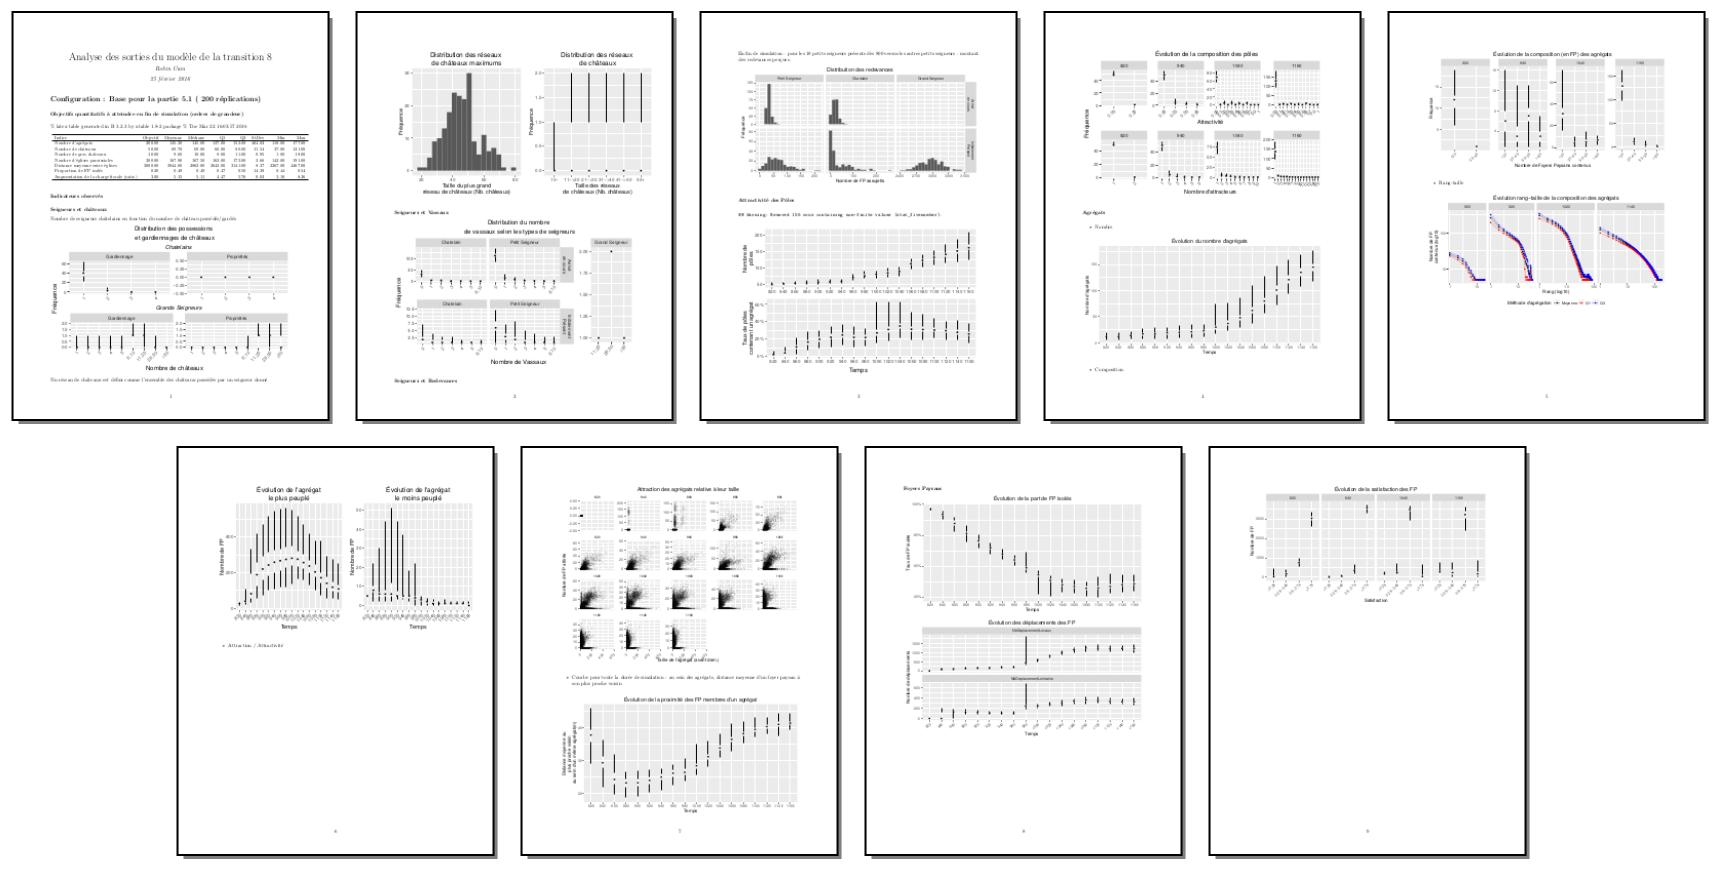
\includegraphics[width=\linewidth]{img/SimFeodal_Rapport_exemple.png}
		\caption{Un exemple de rapport automatique généré pour une expérimentation (étape 0) de SimFeodal. La version en taille réelle est reproduite en \hl{annexe X}.}
		\label{fig:simfeodal_rapport_mini}
	\end{figure}

	\paragraph{Structurer des rapports pour aller vers la reproductibilité des analyses}
	
	Les raisons de ce choix sont multiples. Toutes ont en commun une recherche de reproductibilité des résultats et des analyses menées.
	Une reproductibilité théorique (\hl{encore une ref au positionnement}), puisque les résultats de simulation doivent être analysés et reproduits par des chercheurs potentiellement intéressés.
	Mais cette recherche de reproductibilité est rendue aussi nécessaire par la pratique de la modélisation, tel qu'explicité auparavant (\cref{subsec:capter-replications,subsec:capter-experiences}), faite d'allers-retours qui requièrent une capacité constante à reproduire des résultats déjà observés.
	
	La quantité d'expériences requises pour arriver à un état satisfaisant du modèle est alors importante, et le nombre de rapports tout autant.

	La création d'un rapport automatisé garantit une génération rapide des indicateurs sur les nouvelles données, ce qui permet un examen des sorties de simulation presque immédiatement après leur exécution.
	Cette automatisation permet aussi de mener une seconde évaluation -- après le pré-filtrage constitué par l'observation d'indicateurs en direct -- du bon déroulement \og interne \fg{}\footnote{
		Au sens de l'évaluation interne, c'est-à-dire du bon fonctionnement, exempt de \textit{bugs}, du modèle de simulation implémenté.
	}.
	Le caractère fixe d'un rapport automatisé se base ainsi sur une structure de données contraignante -- par exemple constitués en \textit{n} fichiers dotés de plusieurs colonnes spécifiquement attendues --, dont les caractéristiques sont elles-mêmes contraignantes -- un rapport automatisé ne fonctionnant, par exemple, qu'en présence d'un nombre pré-défini de réplications complètes --.
	En l'absence d'un de ces critères dans des données en sortie de simulations, par exemple si le nombre de réplications est trop faible, le rapport ne peut être généré et émet une erreur.
	La présence ou non de cette erreur constitue donc un nouveau filtre de vérification de la validité du modèle, permettant là encore de détecter des simulations qui présenteraient des comportements incohérents en terme de production de données.

	Un autre intérêt majeur des rapports, déjà pointé en avantage des outils de type \textit{CLI} est leur adaptabilité.
	On a vu (chap. 3) que les indicateurs à examiner sont nombreux et surtout, évolutifs, dans le sens où ces indicateurs ont fortement été modifiés, remplacés, affinés, au cours des étapes de paramétrage de SimFeodal.
	L'utilisation de rapports automatiques permet de modifier le code source -- dont l'exécution génère les indicateurs -- une et une seule fois, c'est-à-dire dans un unique fichier, à une unique position dans le code.
	À partir de là, pour mettre à jour l'ensemble des rapports déjà produits, c'est-à-dire regroupant les indicateurs de chacune des expériences passées, il suffit de ré-exécuter la routine de production des rapports.
	Dans le cas de SimFeodal, caractérisé par de fréquents changements dans la forme et le calcul des indicateurs, cela a représenté un gain de temps et d'efficacité très conséquent.
	Cette démarche devrait donc pouvoir s'appliquer à l'identique, avec les mêmes avantages, dans le cadre plus large de l'évaluation visuelle de modèles.

%	\begin{encadre}{Générer les rapports avec \texttt{R} et \texttt{knitr}}{enc-technique-rapports-knitr}
%
%		\hl{Encadré sur les rapports automatiques, le \textit{\og litterate programming}\fg, le choix et le paramétrage de knitr + lien vers le code-source des rapports.}
%
%	\end{encadre}


	\paragraph{Dépasser les limites de la compatibilité d'ensemble}
	Naturellement, cette préconisation de reproductibilité des rapports constitue plus un objectif théorique à atteindre qu'un retour d'expérience précis tiré des approches d'évaluation mises en place pour le modèle SimFeodal.
	
	Ainsi, comme explicité dans l'encadré sur l'incrémentalité des indicateurs (\hl{ref encadré incrémentalité chap 3}), une contrainte forte empêche une absolue reproductibilité des analyses du comportement des différentes versions de SimFeodal : les données générées par les différentes versions du modèle ne sont pas systématiquement \og compatibles \fg{}, c'est-à-dire qu'elles ne présentent pas toute exactement la même structure, à commencer par les variables enregistrées, quand bien même il aurait été choisi dès le départ d'enregistrer le plus de sorties possibles : le modèle évolue, et avec lui, certaines variables apparaissent et d'autres deviennent caduques.
	La structure contraignante et précise des données nécessaires à la génération des rapports ne peut donc être entièrement satisfaite, et demande une adaptation régulière -- mais aussi rare que possible -- des programmes qui génèrent ces rapports.
	
	On ne peut donc satisfaire globalement à un objectif de reproductibilité, mais il est toutefois possible de limiter la déviance à cette ambition.
	Pour cela, on peut agencer les différentes versions du modèles au sein de \og générations\fg{} de modèle, c'est-à-dire d'ensemble de versions présentant des attributs comparables et générant des données de même structure.
	Plutôt que d'adapter le code-source des rapports à chaque nouvelle version du modèle, ou encore de ne jamais l'adapter et donc d'être tributaire de la structure des toutes premières versions du modèle, cela constitue un choix intermédiaire qui permet de limiter le nombre de variantes de rapports.
	Cette approche suit les grandes lignes du développement logiciel général : les itérations successives d'un logiciel sont constituées de versions \og majeures\fg{} -- les générations de modèles dans notre cas --, qui n'assurent pas nécessairement de compatibilité avec les autres versions majeures, et de versions \og mineures\fg{}, dans lesquelles la compatibilité est assurée\footnote{
		Par exemple, un fichier de dessin vectoriel créé avec le logiciel Adobe Illustrator 15.0 ne sera pas lu correctement avec une version 14.0.
		Ce fichier présentera toutefois un compatibilité parfaite avec les versions 15.1 à 15.\textit{n} du logiciel.
	}.
	
	Pour revenir aux rapports voués à l'évaluation d'un modèle, en inscrivant les différentes versions du modèle -- et des programmes générant les rapport correspondant -- dans des sous-ensemble de versions, les \og générations\fg{}, les différents rapports peuvent être considérés comme reproductibles et automatiques au sein de ces générations.
	Pour SimFeodal, cela implique d'organiser les différentes versions du modèle -- résultant des étapes de paramétrage, \hl{cf. chap4} -- au sein de grandes générations, à chaque changements structurels des mécanismes ou données produites par le modèle.
	
	\paragraph{Les rapports, des instruments suffisants ?}
	
	A l'issue de la conception et de l'implémentation de ces rapports automatiques, on dispose donc, pour chaque expérience, d'un document aisément partageable et lisible.
	Ces documents s'enrichissent, au fur et à mesure des générations de modèles, de nouveaux indicateurs, et sont comparables au sein de ces générations.
	Cela pourrait constituer la dernière étape de la création d'outils d'évaluation d'un modèle, dans la limite d'un nombre de versions ou de génération de modèles assez restreint.
	
	SimFeodal, comme c'est souvent le cas dans les modèles à base d'agent, a toutefois été caractérisé par une forte quantité d'allers-retours entre le modèle et ses résultats, entraînant à chaque fois de nouvelles expérimentations (cf. \cref{sec:sorties-simfeodal}). 
	
	On a vu que la manipulation d'un grand nombre d'indicateurs, même pour une quantité restreinte d'expériences, disqualifiait l'usage de fichiers individuels et poussait à l'usage de rapports structurés.
	Avec un grand nombre d'expériences, les mêmes limites apparaissent pour les rapports : la masse d'expériences rend partiellement caduque l'utilisation unique des rapports automatiques.
	Il est en effet aisé de comparer, sur un même écran d'ordinateur, deux ou trois rapports, mais dès lors qu'il faut en comparer un plus grand nombre, la manipulation conjointe des rapports devient complexe, tout autant que d'avoir une vision globale des résultats principaux de chaque expérience.

	\subsection{Organiser les rapports : Dashboards}\label{subsec:dashboards}

	Pour être en mesure de comparer de nombreux éléments, il est nécessaire de passer d'une exploration linéaire, fondée sur le visualisation successive de chacun des indicateurs, à une exploration globale et interactive.
	En pratique, plutôt que de faire défiler visuellement les nombreuses pages d'indicateurs, mieux vaut une interface présentant les points clefs de l'évaluation et qui permette d'entrer dans le détail de chacun des indicateurs après-coup.

	\subsubsection{Les \textit{dashboards}}

	Cette logique, assez universelle désormais, est celle qui préside à la création des nombreux \og tableaux de bord \fg{}, ou \og \textit{dashboards} \fg{} que l'ont voit émerger depuis la fin des années 1990.
	Rob Kitchin et ses co-auteurs définissent ainsi les \textit{dashboards}, en s'appuyant sur les travaux de Few notamment :

	\begin{quotation}
		\og For Few [\autocite[p.34]{few_information_2006}] a ‘dashboard is
		a visual display of the most important information needed to achieve one or more objectives; consolidated and arranged on a single screen so the information can be monitored at a glance’.
		Just as a car dashboard provides critical information needed to operate the vehicle at a glance, indicator dashboards provide key information for running companies or cities (\st{Dubriwny \& Rivard, 2004}))[\autocite{rivard_are_2004}].\fg{}\\
		\mbox{}~ \hfill \cite[p. 11]{kitchin_knowing_2015}
	\end{quotation}

	Très répandus dans le monde de l'informatique décisionnelle (\textit{Business Intelligence, BI}), ces outils permettent d'explorer des données d'entreprises, par exemple des résultats financiers.
	Pour ce faire, ils mettent en avant, dans une interface unique, des indicateurs clés (\textit{Key Performance Indicators, KPI}), qu'il est ensuite possible de filtrer et d'affiner, par exemple par sélection de différents intervalles temporels.

	Les \textit{KPI} jouent le rôle d'indicateurs synthétiques, c'est-à-dire qu'ils s'adressent à des gestionnaires, par exemple des \textit{managers}, qui ont une expertise importante sur les résultats produits.
	Les utilisateurs des \textit{dashboards} ne sont donc pas des analystes, à même d'explorer eux-mêmes les données mobilisées, mais plutôt des thématiciens qui se fondent sur les indicateurs présentés pour prendre des décisions.

	La dichotomie \og analyste décisionnaire\fg{} s'exprime aussi dans le domaine de la recherche, et notamment dans la recherche en géographie urbaine à visée applicative.
	Avec l'avènement des données massives et de leur prise en compte pour la gestion des villes (\textit{smart cities}), les géographes se sont donc aussi penchés sur des outils de ce type.
	En résulte une utilisation de plus en plus fréquente de \textit{dashboards} en géographie urbaine (\og \textit{city-dashboards}\fg{}, \cite{roumpani_creating_2013, kitchin_knowing_2015, batty_perspective_2015}).

	Le parallèle avec le monde de l'informatique décisionnelle est en effet présent dans les types d'utilisateurs et de producteurs de ces outils : il s'agit de mettre à disposition d'experts thématiques, les décideurs publiques, des indicateurs clés, issus de calculs parfois complexes, afin de leur permettre d'évaluer une situation donnée et de prendre les décisions politiques adéquates.

	Le constat ayant mené à l'apparition des premiers \textit{dashboards}, tant en informatique décisionnelle qu'en géographie urbaine, est identique : les informations nécessaires à l'évaluation d'une situation -- financière, relative aux politiques publiques etc. -- sont de plus en plus nombreuses et hétérogènes.
	Les indicateurs permettant de mener ces évaluations, pensés pour les décideurs qui en feront usage -- managers, acteurs publiques etc. --, se démultiplient et se diversifient aussi par conséquence.

	Inspiré autant par l'usage \textit{BI} que par l'usage géographique, nous considérons que ces outils peuvent se révéler utiles dans l'évaluation de modèles de simulations complexes.
	Les enjeux sont en effet les mêmes : permettre à des thématiciens de comprendre et d'évaluer les sorties d'un modèle, à l'aide d'indicateurs nombreux et complexes présentés de manière transparente relativement à cette complexité.

	Ce positionnement méthodologique s'inscrit pleinement dans la démarche de co-construction interdisciplinaire de SimFeodal.
	On y retrouve ainsi la même logique qui anime les dashboards : une évaluation menée par des thématiciens qui s'appuient pour cela sur des indicateurs clefs (\hl{ref. aux indicateurs les plus importants dans le chap 3}) et précisent leur analyse à l'aide d'indicateurs secondaires présentés sous forme d'un panel varié de visualisations.
	Nous avons donc choisi de ré-organiser les rapports initialement produits pour leur donner une forme plus adaptée à ces enjeux, sous forme de \textit{dashboards}.

	\subsubsection{SimVADB}\label{subsubsec:simvadb}

	Les \textit{dashboards} font souvent usages de représentations graphiques très métaphoriques des tableaux de bords automobiles.
	On y retrouve ainsi fréquemment une forte mise en valeur d'indicateurs numériques simples, par exemple au moyen de jauges (\textit{gauge charts}), de représentation de type thermomètres (\textit{thermometer charts}), ou encore de voyants d'alerte et autres témoins lumineux.
	Pour SimFeodal, les indicateurs étant assez fortement conçus et structurés (\hl{chap. 3}), nous n'avons pas ressenti le besoin de faire appel à ce type de représentation.

	L'usage des dashboards est ainsi plus relatif à l'organisation des indicateurs qu'à leur représentation, qui se voulait aussi semblable que possible à celle qui était déjà produite pour les rapports automatiques.

	Un premier prototype, SimVADB\footnote{
	\textbf{S}imulation \textbf{V}isual \textbf{A}nalysis \textbf{D}ash\textbf{B}oard.\\
	Archive du code-source disponible sur le dépôt Github associé :
	\url{https://github.com/RCura/SimVADB/tree/9a96cc9b6cf59e62e253d6e0859febedda903e03}
	} a ainsi été développé.
	Il s'agissait uniquement de ré-organiser le code source produisant les rapports, au moyen d'outils permettant un affichage sous forme d'application en ligne (Flexdashboard, \autocite{iannone_flexdashboard_2018}).
	Plutôt que de présenter les indicateurs dans des pages successives, on a donc préféré les organiser au seins d'onglets, chaque onglet concernant un type d'entité et présentant l'ensemble des indicateurs propres à ces entités \hl{Faire ref aux captures d'écrans qui seront ajoutées}.\\
	\hl{Refaire tourner cette version de SimVADB pour en faire 2-3 captures d'écran...}\\

	\begin{encadre}{D'un rapport automatique à un \textit{dashboard}}{enc-technique-dashboard}
		\hl{Encadré sur la conversion d'un rapport en un dashboard : logique d'IHM, d'organisation des visus etc.}
	\end{encadre}

	Au niveau de l'interface utilisateur, SimVADB permettait de choisir, dans une liste déroulante, les simulations dont afficher les indicateurs, à partir de leur nom \hl{cf. figure n}.

	Avec la multiplication des valeurs de paramètres testées, il est devenu plus efficace de regrouper les simulations au sein d'expérimentations, dans lesquelles on faisait varier plusieurs paramètres, potentiellement avec de multiples valeurs de paramètres pour chacun.

	À partir de là, il devenait difficile de sélectionner les simulations à partir de leur simple nom, ceux-ci devenant potentiellement complexes, ou recouvrant sinon différentes configurations de paramètres.
	Le choix méthodologique d'interaction avec la plate-forme d'affichage des indicateurs s'est donc révélé inadapté à la sélection et à l'exploration des sorties de SimFeodal.

	Au delà du mode d'interaction, pour évaluer visuellement différentes configurations du modèle, on ne pouvait se contenter d'un simple affichage des données, au sein d'un outil de type présentoir interactif tel que SimVADB.

	Comme dit dans \hl{le chapitre 4}, le paramétrage de SimFeodal a ainsi reposé sur de nombreuses étapes d'évaluation des différentes version du modèle.
	Pour cela, l'approche principale a été la comparaison, point par point, entre les résultats des indicateurs de sortie de simulation des versions successives de SimFeodal.

	Un outil de présentation statique des résultats n'est pas un outil de comparaison.
	S'il suffit pour de la restitution, par exemple dans le cadre du rapport systématique des résultats de SimFeodal, on ne peut s'appuyer uniquement sur une succession d'évaluations visuelles pour appréhender l'étendue des changements apportées par une modification des valeurs de paramètres.

	\subsection{Interagir avec les rapports : exploration interactive}\label{subsec:explo-interactive}

	Face à la démultiplication des expérimentations, consécutive aux nombreuses étapes de paramétrage de SimFeodal (\hl{cf. chap 4}), il a donc fallu repenser la plate-forme d'évaluation des résultats.
	Pour cela, considérant que les simulations ne pouvaient être aisément appréhendées et sélectionnées par leur nom, numéro d'étape ou de version, il a été décidé d'adopter une posture plus proche de l'exploration de modèle en elle-même.
	C'est-à-dire de ne pas caractériser les simulations par un identifiant quelconque, mais plutôt par leur spécificité intrinsèque, c'est-à-dire la combinaison de valeurs de paramètres qui les rendent uniques.
	Ce faisant, au sein de la plate-forme d'exploration, SimVADB, l'enjeu devenait ainsi plutôt la compréhension des effets des valeurs de paramètres sur les indicateurs que l'évaluation visuelle d'une simulation en particulier.
	Du point de vue de l'interface utilisateur, cela implique que la sélection ne se fasse plus par un unique critère (le nom de la simulation), mais par une succession de sélection, chaque paramètre constituant un nouveau filtre dans lequel choisir les valeurs à interroger.

	La quantité de paramètres en entrée étant importante (\hl{cf. plus haut}), et pouvant dès lors donner lieu à un mode de sélection complexe et fastidieux -- définir une par une les valeurs voulues pour chacun des 45 paramètres --, nous avons choisi encore une fois de nous appuyer sur l'aspect visuel afin de permettre aux utilisateurs de SimVADB de choisir la ou les expérimentations à analyser.

	Pour cela, on a choisi de représenter les combinaisons de paramètres dans un graphique en \og coordonnées parallèles \fg{} (\textit{parallel coordinates}, d'après \cite{inselberg_parallel_1987}, voir \cite{few_multivariate_2006} par exemple pour une description plus succincte, illustrée et pratique) :
	ce type de graphique est en effet extrêmement pertinent pour représenter une information multi-dimensionnelle en ce qu'il permet de détecter graphiquement des \textit{cluster} de lignes \autocite[2]{heinrich_state_2013}, c'est-à-dire de faire ressortir visuellement les expériences dont les valeurs de paramètre sont proches.


	\begin{encadre}{Construction et utilisation interactive d'un graphique en coordonnées parallèles}{parcoords}

			\begin{figure}[H]
			\captionsetup{width=\linewidth}
			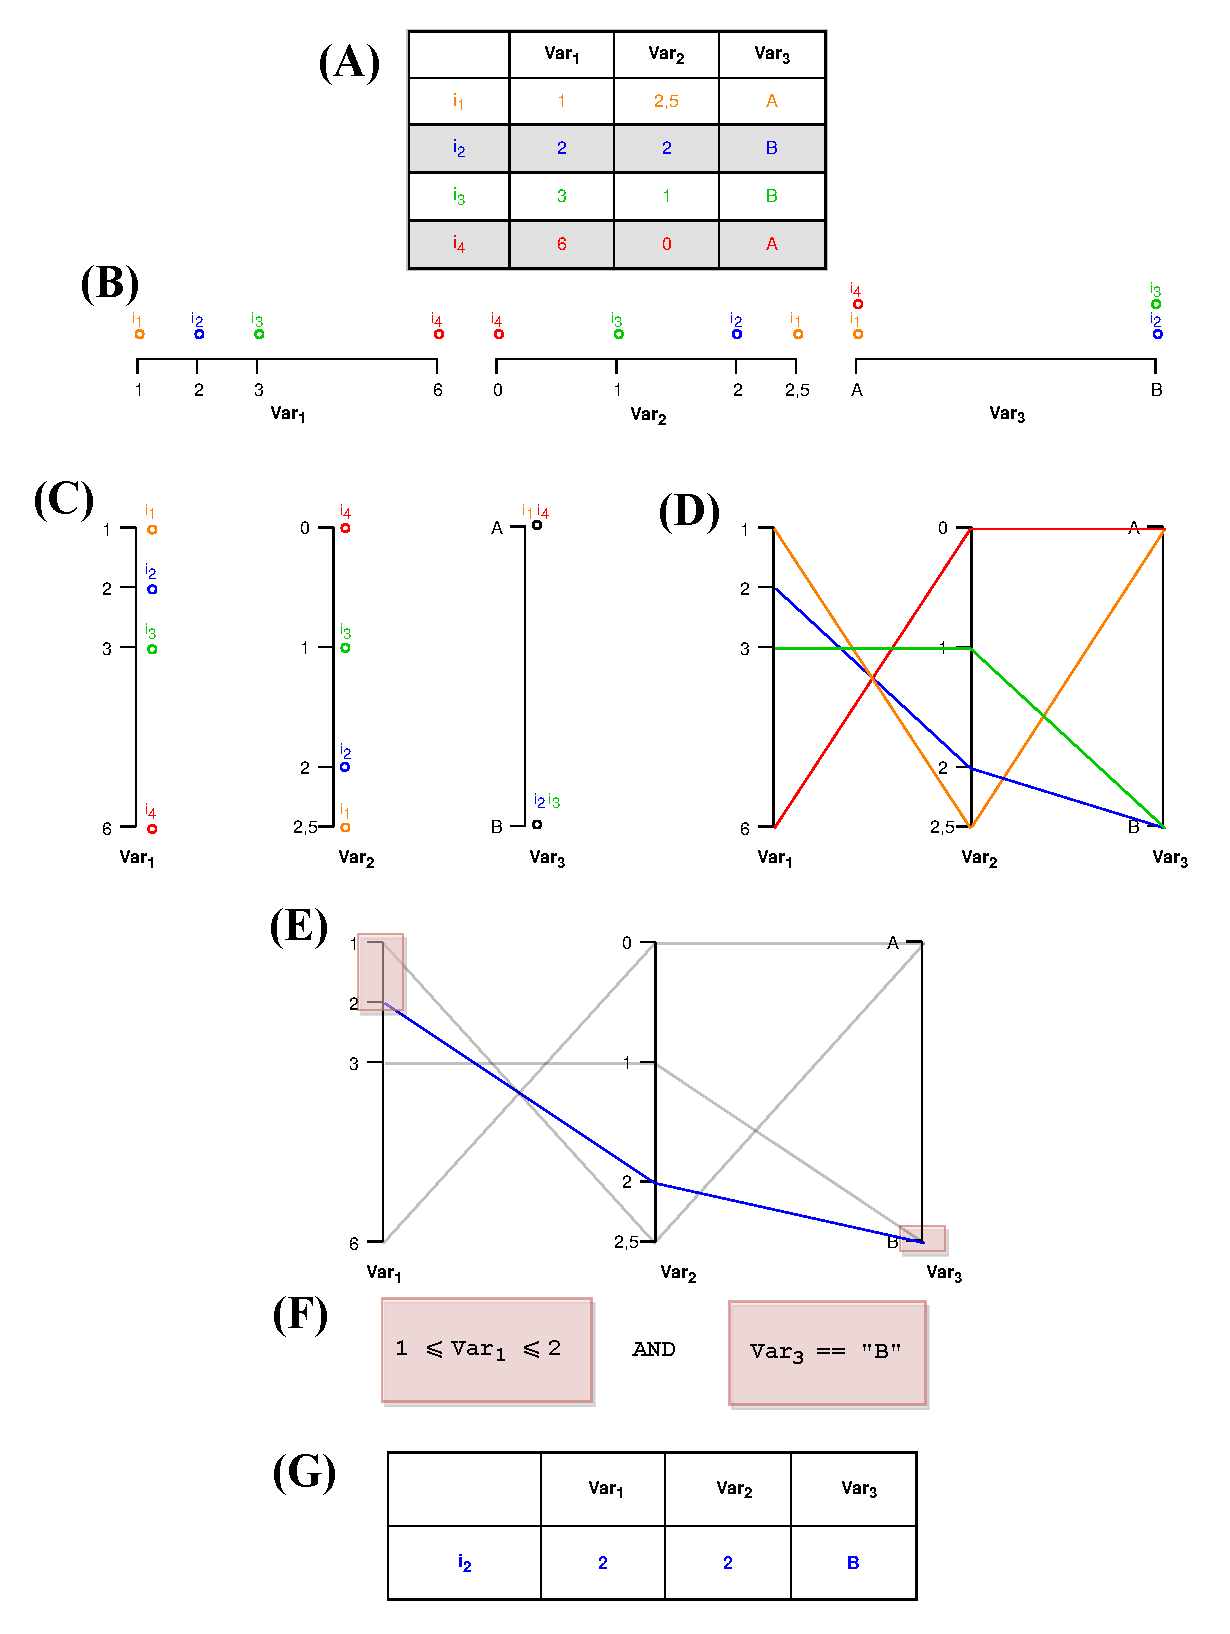
\includegraphics[width=\linewidth]{img/ParCoords_Brush.pdf}
			\caption{Démarche de construction d'un graphique en coordonnées parallèles (\textbf{A}--\textbf{D}) et sélection par \textit{brushing} (\textbf{E}--\textbf{G}).}
			\label{fig:schema_parcoords}
		\end{figure}

	\end{encadre}



	De plus, en matière d'interaction, on utilise fréquemment les graphiques en coordonnées parallèles en vue de filtrage, le plus souvent par des actions de \textit{brushing} (\og brossage\fg{}, c'est-à-dire sélection graphique d'une zone en dessinant son étendue à la souris -- cf. \cref{enc:parcoords}).
	Ce type de sélection se révèle en effet souvent plus efficace et intuitive qu'une sélection textuelle plus systématique :

	\begin{quotation}
		\og Filtering is an operation that removes signals from its input. A filter reduces the number of lines to be rendered. In this sense, dynamic querying [...] is a filter, if implemented with brushing [...], which reduces clutter by putting the filtered lines in focus using some highlighting mechanism. Combining simple brushes using logical operators [...] further allows the user to formulate rather complex queries that might even achieve faster and more accurate results using parallel coordinates than using a Structured Query Language (SQL) [...].\fg{}\\
		\mbox{}~ \hfill \cite[p. 13]{heinrich_state_2013}
	\end{quotation}

	Cette utilisation est aussi courante en géographie quantitative, et on la retrouve par exemple chez l'un des représentants de l'analyse spatiale des années 1990, Stewart Fotheringham, qui indique même l'usage du graphique en coordonnées parallèles en tant que filtre pour identifier des informations dans une autre dimension, spatiale ici : \og the data being displayed in parallel coordinates can be linked to a map and then brushed to highlight the locations of interesting lines displayed in \textit{m}-space on the parallel co-ordinates.\fg{} \autocite{fotheringham_trends_1999}.

	Appliqué aux données de SimFeodal, cette interface (\cref{fig:simvadb_dashboard}) se révèle particulièrement efficace pour sélectionner les configurations de paramètres à explorer.
	Ainsi, en \og brossant \fg{} quelques filtres manuellement (\cref{fig:simvadb_dashboard} - \textbf{A}), on arrive rapidement à isoler une expérience spécifique.

	\begin{figure}[H]
		\captionsetup{width=\linewidth}
		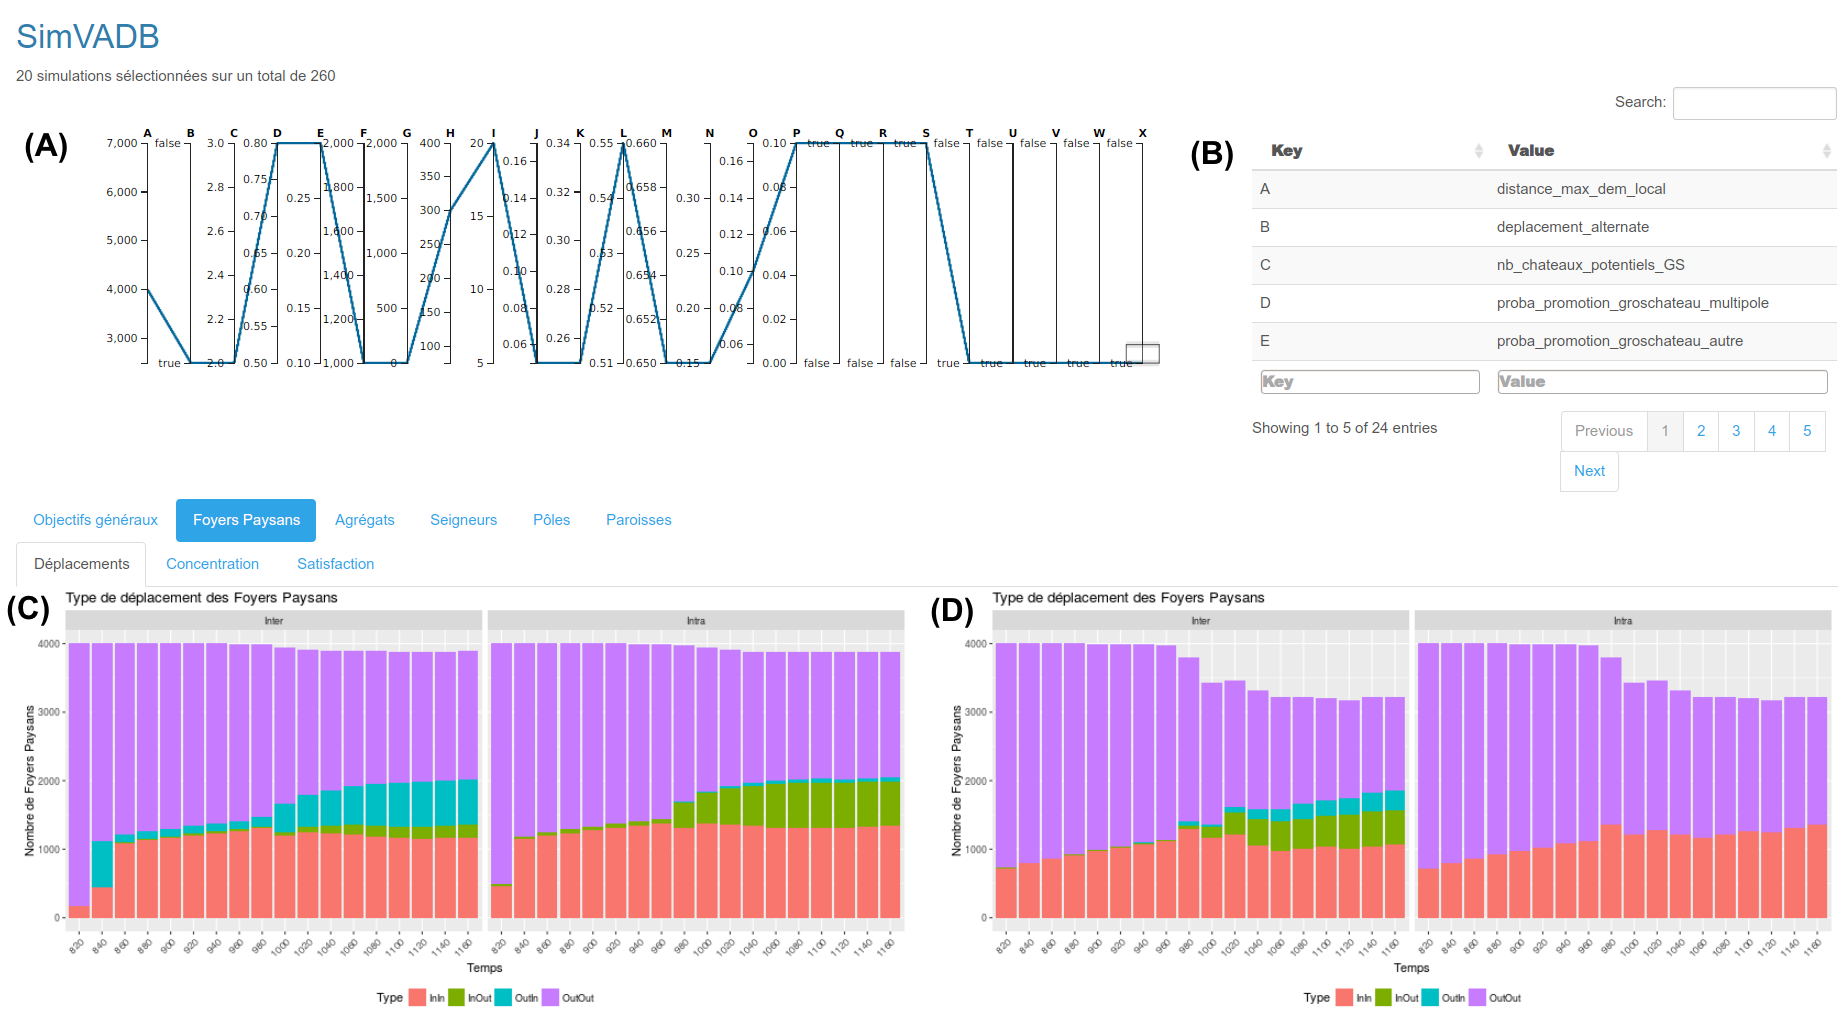
\includegraphics[width=\linewidth]{img/SimVADB_Dashboard2_annote.png}
		\caption{SimVADB (Simulation Visual Analysis DashBoard), un \textit{dashboard} d'exploration visuelle des indicateurs de sortie de simulation de SimFeodal.\\
		La sélection des simulations à explorer se fait dans le graphique en coordonnées parallèles (\textbf{A}), en \og brossant\fg{} des filtres graphiques sur les \og dimensions\fg{} du graphique, dimensions dont les intitulés sont explicités dans le tableau \textbf{B}.
		Les graphiques \textbf{C} et \textbf{D} indiquent l'évolution des types de déplacements des foyers paysans au cours des simulations.\\
		- Le graphique \textbf{C} représente, pour cet indicateur, une moyenne de l'ensemble des simulations intégrées dans la base de données (260 ici), recouvrant donc plusieurs valeurs de paramètres.\\
		- Le graphique \textbf{D} représente cet indicateur calculé depuis un sous-ensemble de 20 simulations (donc une expérience composée de 20 réplications), pour lesquelles le paramètre \og \texttt{X} \fg{}(\hl{Retrouver nom de ce paramètre}) vaut \texttt{true}.}
		\label{fig:simvadb_dashboard}
	\end{figure}

	Afin de permettre aux utilisateurs de remarquer les particularités des simulations explorées, nous avons choisi de mettre en emphase les différences entre la tendance générale des indicateurs, en calculant des moyennes de l'ensemble des simulations (\cref{fig:simvadb_dashboard} - \textbf{C}), et les valeurs spécifiques des indicateurs de l'expérience choisie (\cref{fig:simvadb_dashboard} - \textbf{D}).
	Cela permet, visuellement, d'être en mesure d'évaluer les sorties de simulation d'une expérience tout en ayant un référentiel visible.
	Les différentes expériences produisent des résultats sensiblement similaires\footnote{
		Si chaque expérience, et chaque réplication, produisent des résultats uniques, le choix d'une évaluation par des indicateurs visuels peut prêter à confusion si l'on n'a pas de repère précis.
		Les critères attendus, présentés dans \hl{le chapitre 3} sont ainsi assez précis pour départager une simulation très éloignée des attentes et une autre simulation plus conforme.
		Pour autant, par exemple quand les valeurs de paramètres varient faiblement, les résultats produits peuvent être assez similaires dans les grandes tendances qu'ils font ressortir.

	}, et on ne peut alors plus les comprendre sans les confronter à d'autres résultats similaires.
	Le choix d'une agrégation de l'ensemble des simulations effectuées est discutable, en ce qu'on aurait par exemple pu plutôt isoler des simulations \og de référence \fg{} afin de diminuer l'effet \og d'aplatissement \fg{} engendré par l'agrégation de résultats nombreux et hétérogènes.
	Toutefois, la variabilité des résultats étant encore assez restreinte, au moment de la création et de l'utilisation de SimVADB, ce référentiel agrégé permettait déjà une compréhension plus fine des sorties de simulations, en particulier dans l'analyse de l'impact de variations fines de valeurs de paramètres.

	\subsection{Explorer en comparant : SimEDB}\label{subsec:explorer-simedb}

	Après le travail de paramétrage grossier qui a permis de stabiliser les mécanismes, le paramétrage de SimFeodal est entré dans une phase plus fine, visant à mieux calibrer le modèle à l'aide de variations de valeurs de paramètres de granularité inférieures.

	Dans ce cadre, par exemple en faisant varier le nombre de foyers paysans de $4000$ à $4200$ ($5\%$ de variation), les résultats du modèle changent peu :  de faibles variations de valeurs de paramètres entraînent le plus souvent de faibles variations dans les indicateurs de sorties observés\footnote{
	On peut de plus noter que, les variations n'étant pas linéaires, les répercussions d'un changement de valeur de paramètre peuvent être très différentes de l'ordre de grandeur de ce changement de valeur. Par exemple, pour ces $5\%$ de variation dans le nombre de foyers paysans, la majorité des indicateurs variera de moins de $1\%$.
	}.
	En vue d'évaluer les simulations, et donc de les différencier les unes des autres à l'aune des indicateurs générés, la comparaison d'une expérience spécifique avec un référentiel constitué de toutes les expériences précédentes ne permet plus de mener ce travail de comparaison fine : par rapport à une référentiel unique, qu'il soit constitué d'une agrégation de simulations ou même d'une version \og de base\fg{} du modèle (par exemple les versions principales identifiées dans le \hl{chapitre 4}), les variations sont trop fines pour être distinguables les unes des autres.

	Pour pouvoir correctement évaluer les apports d'un nouveau jeu de valeurs de paramètres, et donc, dans une démarche itérative, pouvoir différencier deux expériences successives, il est donc nécessaire d'être en mesure de comparer directement les expériences les unes avec les autres.
	Il est donc indispensable de ne plus mener une comparaison visuelle entre un référentiel commun et une expérience spécifique, mais bien de baser l'évaluation sur la comparaison entre cette expérience spécifique et une autre expérience, tout aussi spécifique.
	D'un point de vue méthodologique, cela requiert de pouvoir afficher conjointement les indicateurs de sorties de deux expériences isolées de la masse des simulations.
	La sélection d'une expérience via l'usage de \textit{brushing} sur un graphique en coordonnées parallèles des valeurs de paramètres ayant montré son efficacité, il a été choisi d'étendre ce principe d'interactivité au choix du référentiel, c'est-à-dire de baser l'évaluation non plus sur la sélection d'une expérience spécifique, mais de deux expériences spécifiques.

	\begin{figure}[H]
		\centering
		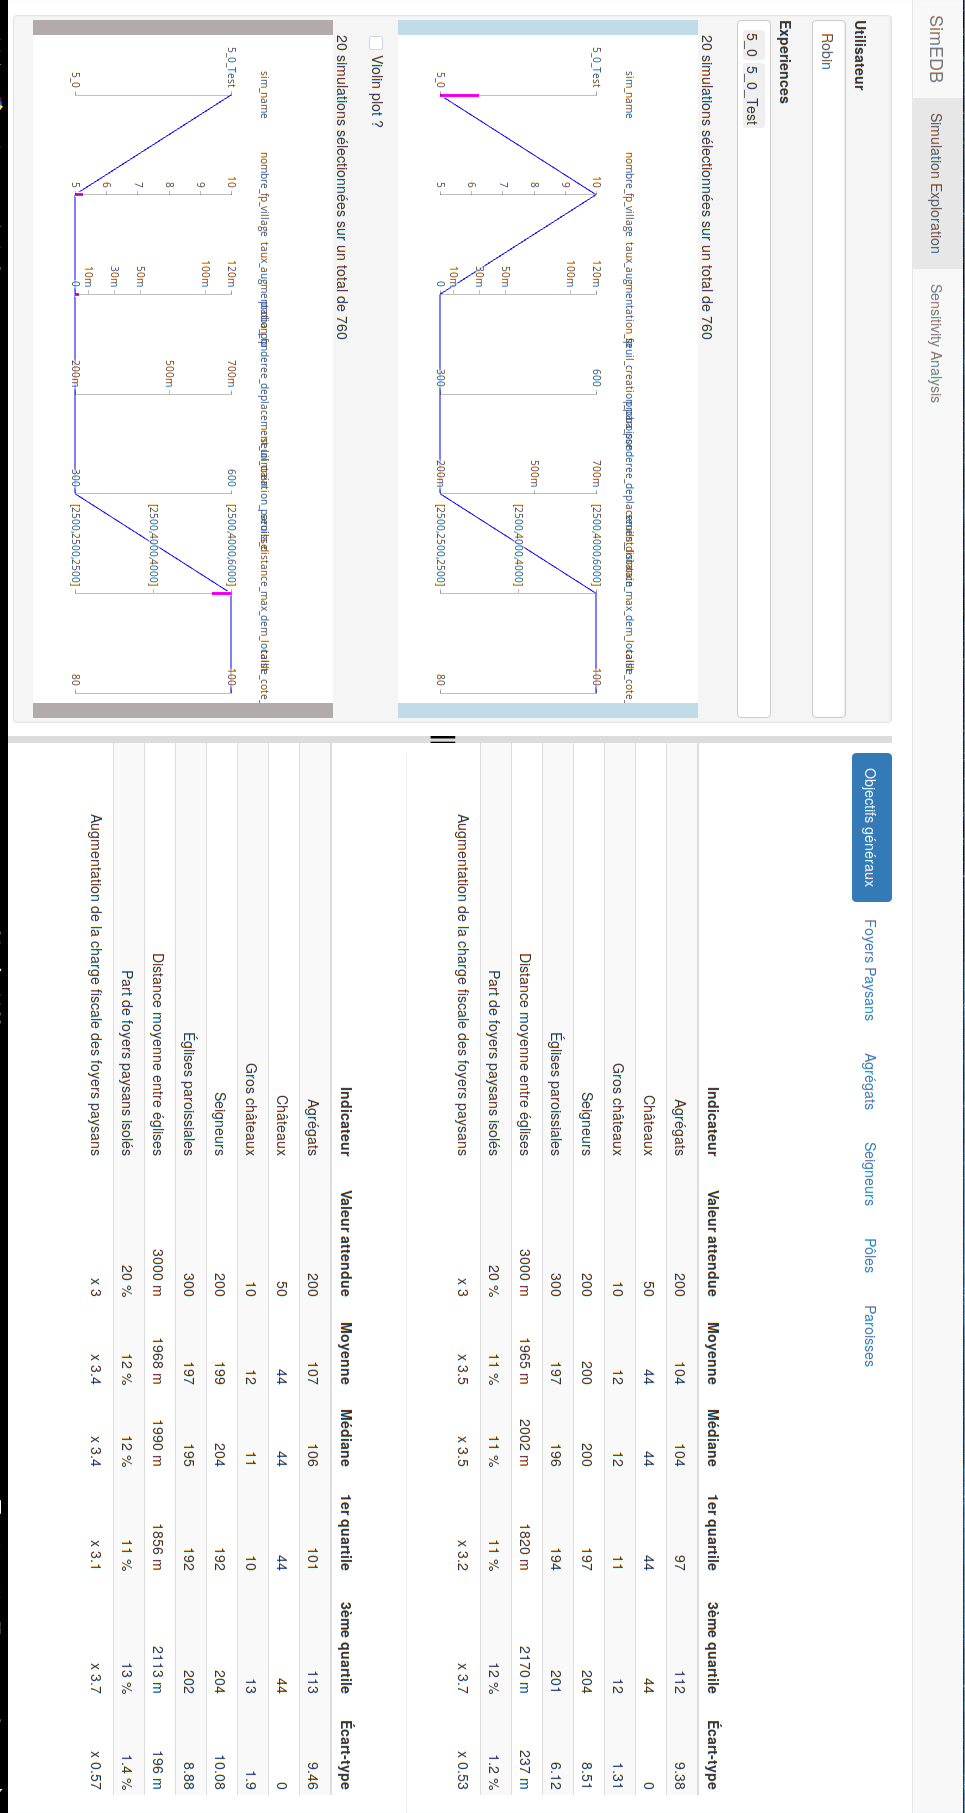
\includegraphics[width=.94\linewidth]{img/SimEDB_nombreFP_villages_rotate.png}
		\caption{SimEDB }
		\label{fig:simedb_villages}
	\end{figure}
\clearpage

	Dans cette version remaniée de la plate-forme d'exploration, renommée pour l'occasion SimEDB\label{par:introduction-nom-simedb} (\textbf{Sim}Feodal \textbf{E}xploration \textbf{D}ash\textbf{B}oard)\footnote{\label{ftn:origine-simedb}
		La plate-forme d'exploration SimVADB (SimFeodal Visual Analysis Dashboard) a été renommée SimEDB ([...] Exploration Dashboard) par soucis de simplicité, le terme \og Exploration\fg{} nous semblant plus compréhensible et explicite que celui de Visual Analysis. Cela permet de plus une cohérence sémantique entre plusieurs productions de l'auteur -- TimeLineEDB - \autocite{cura_timelineedb_2017}; RoadTrafficEDB et CitiBikeEDB - \autocite{cura_making_2017} --, inscrivant cette plate-forme d'exploration de données issues de simulation dans une \og famille \fg{} d'outils d'exploration de données spatio-temporelles.
	}, l'accent est donc mis sur la comparaison de deux ensembles de résultats, chacun répondant à une sélection propre.
	En superposant les graphiques et tableaux des indicateurs, la comparaison visuelle est facilitée.
	On peut alors aussi bien comparer deux variations fines d'un mécanisme -- en sélectionnant par exemple une unique différence dans les valeurs de paramètres (par exemple le nombre de foyers paysans présents à l'initialisation du modèle dans les villages (\cref{fig:simedb_villages}))) --, ou encore comparer les différences entre une version stable et les expériences en découlant -- en sélectionnant, par exemple dans la partie supérieure, une version que l'on estime suffisamment aboutie pour constituer un référentiel, et dans la partie inférieure, une série d'expériences issues de ce référentiel et qui font varier plusieurs paramètres.


	\paragraph*{}
	Nous reviendrons plus précisément et longuement sur la description de SimEDB dans les parties suivantes (\cref{sec:SimEDB}, p. \pageref{sec:SimEDB}), mais après en avoir décrit les étapes de construction et les besoins auxquelles ces évolutions répondaient, il est maintenant nécessaire de revenir sur les données manipulées par cette plate-forme d'exploration.
	Le type, la structure et la masse de ces données (\cref{sec:sorties-simfeodal}) sont en effet indissociables des choix méthodologiques effectués pour SimEDB.
	Il est donc important de présenter les choix et contraintes de ces données avant d'entrer dans une description approfondie de la plate-forme.
